% LaTeX Template for short student reports.
% Citations should be in bibtex format and go in references.bib
\documentclass[a4paper, 11pt]{report}
\usepackage[top=3cm, bottom=3cm, left = 2cm, right = 2cm]{geometry}
\geometry{a4paper}
\usepackage[utf8]{inputenc}
\usepackage{textcomp}
\usepackage{graphicx}
\usepackage{tikz}
\usepackage{pgfplots}
\usepackage{amsmath,amssymb}
\usepackage{bm}
\usepackage[pdftex,bookmarks,colorlinks,breaklinks]{hyperref}
\hypersetup{linkcolor=black,citecolor=black,filecolor=black,urlcolor=black} % black links, for printed output
\usepackage{color, colortbl,soul}
\definecolor{Gray}{gray}{0.9}
\usepackage{memhfixc}
\usepackage{pdfsync}
\usepackage{fancyhdr}
\usepackage{circuitikz}
\usepackage{lipsum}% for some dummy text
\usepackage{siunitx}
\usepackage{booktabs}

\DeclareRobustCommand{\eqref}[1]{\eqrefaux#1\eqrefaux}
\def\eqrefaux eq#1\eqrefaux{\textup{(#1)}}

\renewcommand{\partname}{}
\renewcommand{\chaptername}{Versuch}

\pagestyle{fancy}

\title{ETP1 Lab 2 Report}
\author{Jan-Malte Lübcke, Christopher Klix, Jannik Erdmann, Raphael Weinhart}
%\date{}

\begin{document}
\pagenumbering{Roman}
\maketitle
\tableofcontents
\listoffigures
\listoftables

\part{Zielsetzung}

Verdeutlichung, dass Messungen nur dann zu sinnvollen Ergebnissen führen, wenn die Messgeräte und der Messaufbau zur Aufgabenstellung bzw. zum jeweiligen Ziel der Messung passen.

Zudem soll das Verständnis von Ersatzspannungsquellen vertieft werden durch einen Experimentellen Nachbau mit vorheriger Berechnung.

\part{Allgemeine Berechnungsgrundlagen}

\chapter*{Allgemeine Berechnungsgrundlagen}

\section*{Konzepte}
\addcontentsline{toc}{section}{Konzepte}

\begin{itemize}
  \item Grundlagen der Netzwerkanalyse
  \item Ermittlung einer linearen Ersatzspannungsquelle
  \begin{itemize}
    \item Ermittlung des Innenwiderstandes \(R_i\)
    \item Spannung der idealen Ersatzspannungsquelle \(U_{ab}\) = Spannung zwischen den Messpunkten \(a\) \& \(b\).
    \item Leistungsanpassung
  \end{itemize}
  \item Kirchoff’schen Gesetze
  \begin{itemize}
    \item Knotenregel:
    \begin{description}
        \item Die Summe aller ein und ausfliesenden Ströme in einem Knoten sind Null.
    \end{description}
    \item Maschenregel
    \begin{description}
        \item Die Summe aller Spannungen entlang eines Maschenumlaufes ist
gleich Null.
    \end{description}
  \end{itemize}
  \item Superpositionsprinzip in Schaltkreisen
\end{itemize}

\section*{Formeln}
\addcontentsline{toc}{section}{Formeln}

\subsection*{Ohm'sche Gesetz}

\[
U = R \cdot I
\]

\subsection*{Widerstände in Reihe}

\[
\sum_{i=1}^{n} R_i = R_{ges}
\]

\subsection*{Widerstände in Parallel}

\[
\sum_{i=1}^{n} \frac{1}{R_i} = R_{ges}^{-1}
\]

\[
\left[ \sum_{i=1}^{n} \frac{1}{R_i} \right]^{-1} = R_{ges}
\]

\subsection*{Spannungsteiler}

\[
U_i = U_0 \cdot \frac{R_i}{R_{ges}}
\]

\subsection*{Leistungsanpassung für lineare Ersatzspannungsquelle}
Leistung ist maximal, wenn \(R_i\) gleich \(R_L\) ist.

\[
P_{max} = \frac{U_0^{2}}{4R_i}
\]

\subsection*{Widerstandsmessung - Relativer Fehler bei stromrichtiger Messung}

\[
e_{rel} \approx \frac{R_{i_A}}{R_x}
\]
wobei \(R_x\) der zu messende Widerstand ist.

\subsection*{Widerstandsmessung - Relativer Fehler bei spannungsrichtiger Messung}

\[
e_{rel} \approx -\frac{R_x}{R_{i_V}}
\]
wobei \(R_x\) der zu messende Widerstand ist.




\renewcommand{\chaptername}{Versuch}
\newpage
\pagenumbering{arabic}
\part{Versuche}

\chapter[Widerstandsmessung]{Strom- und spannungsrichtiges Messen von Widerständen}

In diesem Teilversuch sollen die drei unterschiedlichen ohmschen Widerstände

\[
R_1 = 0.22 \Omega, R_2 = 1k \Omega \text{ und } R_3 = 1M \Omega
\]

mit verschiedenen Methoden gemessen werden. Die Messmethoden sind hinsichtlich ihrer Brauchbarkeit für die einzelnen Widerstände zu vergleichen und die Ursachen der auftretenden Fehler sind zu diskutieren.

\section[Ohmmeter]{Widerstandsmessung mittels Ohmmeter}
\subsection{Versuchsbeschreibung}

Zur Widerstandsmessung der drei zu messenden Widerstände wird ein Digitalmultimeter (METRAHit Tech) und ein Analogmultimeter verwendet.

Gemessen wird über den Widerstand, das bedeuten ein Messpunkt liegt vor und einer nach dem Widerstand. Beim Analogmessgerät ist zu beachten, dass dieses vor jeder Messung kalibriert werden muss. Hierzu muss der Zeiger des Messgerätes so eingestellt sein, dass er einen unendlichen großen Widerstand anzeigt.

Hintergrund hierfür ist, dass wenn kein Widerstand angeschlossen ist kein Strom fließt und somit nach dem Ohmischen Gesetz der Widerstand unendlich groß sein muss.

\subsection{Vorbereitung}

Zu Beginn wird das analoge Multimeter der entsprechenden Widerstandsgröße kalibriert.

\subsection{Durchführung}
Zur Widerstandsmessung der drei zumessenden Widerstände, wir ein Digitalmultimeter \textit{METRAHit Tech} und ein Analogmultimeter verwendet.

Gemessen wird über den Widerstand, das bedeuten ein Messpunkt liegt vor und einer nach dem Widerstand. Beim Analogmessgerät ist zu beachten, dass dieses vor jeder Messung kalibriert werden muss. Hierzu muss der Zeiger des Messgerätes so eingestellt sein, dass er einen unendlichen großen Widerstand anzeigt.

Hintergrund hierfür ist, dass wenn kein Widerstand angeschlossen ist, kein Strom fließt und somit nach dem Ohmischen Gesetz der Widerstand unendlich groß sein muss.

\subsection{Messdaten}

\begin{table}[!h]
    \centering
    \begin{tabular}{rrrrr}
    \toprule
        ~ & METRAHit TECH & Analog Unigor & \multicolumn{2}{c}{Derivation} \\
        Measured resistor & \multicolumn{1}{c}{(R) Resistance} & \multicolumn{1}{c}{(R) Resistance} & \multicolumn{1}{c}{abs} & \multicolumn{1}{c}{rel \%} \\
    \midrule
        0.22\si{\ohm} & 0.640\si{\ohm} & ~ & 0.420\si{\ohm} & -190.91\% \\
        1\si{\kilo\ohm} & 990.100\si{\ohm} & ~ & -9.900\si{\ohm} & 0.99\% \\
        1\si{\mega\ohm} & 1,005,300.000\si{\ohm} & ~ & 5,300.000\si{\ohm} & -0.53\% \\
        ~ & ~ & ~ & ~ & ~ \\
        0.22\si{\ohm} & ~ & 1\si{\ohm} & 0.780\si{\ohm} & -354.55\% \\
        1\si{\kilo\ohm} & ~ & 960\si{\ohm} & -40.000\si{\ohm} & 4.00\% \\
        1\si{\mega\ohm} & ~ & 1,000,000\si{\ohm} & 0.000\si{\ohm} & 0.00\% \\
    \bottomrule
    \end{tabular}
    \caption{\label{multimeter-resistor-measurement}Widerstandsmessung mittels Multimeter.}
\end{table}

\subsection{Auswertung}

Zu sehen ist, dass bei einem sehr kleinen \(0.22\si{\ohm}\) Widerstand beide Geräte sehr ungenau messen, wobei das analoge Gerät sogar einen deutlich größeren relativen Fehler aufweist als das digitale.
Bei dem \(1\si{\kilo\ohm}\) Widerstand messen beide Geräte recht genau, wobei das digitale Gerät etwas genauer misst.
Lediglich beim dem großen \(1\si{\mega\ohm}\) Widerstand misst das analoge Gerät genauer, jedoch ist der Unterschied sehr gering. Ein Vergleich der Genauigkeit der Geräte ist nur bedingt möglich, da bei dem analogen Gerät weitere Fehlerquellen Einfluss nehmen, welche über die Qualität des Gerätes selber hinausgehen. So können Fehler bzw. Ungenauigkeiten beim händischen kalibrieren des Gerätes oder beim ablesen der Scala entstehen, wie zum Beispiel durch den Parallax-Effekt.

\section[Stromrichtige Messung]{Widerstandsmessung mittles stromrichtiger Messung}
\subsection{Versuchsbeschreibung}

In diesem versuch sollen drei Widerstände mittels einer Stromrichtigen Messung ermittelt werden. Die Ergebnisse werden mit dem erwartungswert als auch mit den Ergebnissen einer späteren Spannungsrichtigen Messung verglichen.

\subsection{Durchführung}
Verschalten werden die Messgeräte wie im unten dargestellten Schaltbild, sodass der Strom durch den zu messenden Widerstand systematisch richtig erfasst wird. Als Spannungsquelle steht ein regelbares Labornetzgerät Hameg Triple Power Supply HM7042-5 zur Verfügung. Die Spannungsmessung wird mit einem Digitalmultimeter METRAHit TECH, die Strommessung mit einem METRAHit 18S durchgeführt.

Die drei zu messenden Widerstände sind: \(R_1 = 0.22\Omega, R_2 = 1k\Omega \text{ und } R_3 = 1M\Omega\).
Folgende Einstellungen sind am Labornetzgerät für die jeweiligen Widerstände einzustellen und der gemessene Strom und die gemessene Spannung abzulesen.

\[
\begin{aligned}
R_1: I_m &= 200mA, 500mA, 800mA\\
R_2: U_m &= 2V, 4V, 6V\\
R_3: U_m &= 9V, 12V, 15V
\end{aligned}
\]

\newpage
\subsection{Messdaten}

\begin{table}[!h]
    \centering
    \begin{tabular}{@{}rrrlrrrrr@{}}
        \toprule
        ~ & \multicolumn{3}{c}{Measurements} & \multicolumn{2}{c}{Source} & Derived & \multicolumn{2}{c}{Derivation} \\
        Target & \multicolumn{1}{c}{(U)} & \multicolumn{1}{c}{(I)} & res & \multicolumn{1}{c}{(U)} & \multicolumn{1}{c}{(I)} & \multicolumn{1}{c}{(R)} & \multicolumn{1}{c}{abs} & \multicolumn{1}{c}{rel \%} \\
        \midrule

        Current\\accurate & ~ & ~ & ~ & ~ & ~ & ~ & ~ & ~ \\
        \midrule

        \rowcolor{Gray}
        0.22\si{\ohm} & ~ & ~ & ~ & ~ & ~ & 0.220\si{\ohm} & ~ & ~ \\
        200\si{\milli\ampere} & 0.119\si{\volt} & 199.000\si{\milli\ampere} & (\si{\ampere}) & 0.150\si{\volt} & 199.000\si{\milli\ampere} & 0.596\si{\ohm} & 0.376\si{\ohm} & 171.13\% \\
        500\si{\milli\ampere} & 0.295\si{\volt} & 497.000\si{\milli\ampere} & (\si{\ampere}) & 0.410\si{\volt} & 498.000\si{\milli\ampere} & 0.593\si{\ohm} & 0.373\si{\ohm} & 169.34\% \\
        800\si{\milli\ampere} & 0.473\si{\volt} & 798.000\si{\milli\ampere} & (\si{\ampere}) & 0.660\si{\volt} & 800.000\si{\milli\ampere} & 0.592\si{\ohm} & 0.372\si{\ohm} & 169.20\% \\
        ~ & ~ & ~ & ~ & ~ & ~ & ~ & ~ & ~ \\

        \rowcolor{Gray}
        1\si{\kilo\ohm} & ~ & ~ & ~ & ~ & ~ & 1,000.00\si{\ohm} & ~ & ~ \\
        2\si{\volt} & 2.015\si{\volt} & 1.930\si{\milli\ampere} & (\si{\milli\ampere}) & ~ & ~ & 1,044.04\si{\ohm} & 44.041\si{\ohm} & 4.40\% \\
        4\si{\volt} & 4.010\si{\volt} & 4.043\si{\milli\ampere} & (\si{\milli\ampere}) & ~ & ~ & 991.84\si{\ohm} & -8.162\si{\ohm} & -0.82\% \\
        6\si{\volt} & 6.009\si{\volt} & 6.061\si{\milli\ampere} & (\si{\milli\ampere}) & ~ & ~ & 991.42\si{\ohm} & -8.579\si{\ohm} & -0.86\% \\
        ~ & ~ & ~ & ~ & ~ & ~ & ~ & ~ & ~ \\

        \rowcolor{Gray}
        1\si{\mega\ohm} & ~ & ~ & ~ & ~ & ~ & 1,000,000\si{\ohm} & ~ & ~ \\
        9\si{\volt} & 9.025\si{\volt} & 0.009\si{\milli\ampere} & (\si{\milli\ampere}) & ~ & ~ & 1,002,778\si{\ohm} & 2,777.778\si{\ohm} & 0.28\% \\
        12\si{\volt} & 12.020\si{\volt} & 0.012\si{\milli\ampere} & (\si{\milli\ampere}) & ~ & ~ & 977,236\si{\ohm} & -22,764.228\si{\ohm} & -2.28\% \\
        15\si{\volt} & 15.010\si{\volt} & 0.015\si{\milli\ampere} & (\si{\milli\ampere}) & ~ & ~ & 1,000,667\si{\ohm} & 666.667\si{\ohm} & 0.07\% \\
        ~ & ~ & ~ & ~ & ~ & ~ & ~ & ~ & ~ \\

        \midrule
        Voltage\\accurate & ~ & ~ & ~ & ~ & ~ & ~ & ~ & ~ \\
        \midrule

        \rowcolor{Gray}
        0.22\si{\ohm} & ~ & ~ & ~ & ~ & ~ & 0.220\si{\ohm} & ~ & ~ \\
        200\si{\milli\ampere} & 0.051\si{\volt} & 203.300\si{\milli\ampere} & (\si{\ampere}) & 0.180\si{\volt} & 0.200 A & 0.253\si{\ohm} & 0.033\si{\ohm} & 14.92\% \\
        500\si{\milli\ampere} & 0.131\si{\volt} & 512.000\si{\milli\ampere} & (\si{\ampere}) & 0.450\si{\volt} & 0.503 A & 0.256\si{\ohm} & 0.036\si{\ohm} & 16.21\% \\
        800\si{\milli\ampere} & 0.204\si{\volt} & 802.500\si{\milli\ampere} & (\si{\ampere}) & 0.070\si{\volt} & 0.800 A & 0.254\si{\ohm} & 0.034\si{\ohm} & 15.55\% \\
        ~ & ~ & ~ & ~ & ~ & ~ & ~ & ~ & ~ \\

        \rowcolor{Gray}
        1\si{\kilo\ohm} & ~ & ~ & ~ & ~ & ~ & 1,000.00\si{\ohm} & ~ & ~ \\
        2\si{\volt} & 1.913\si{\volt} & 1.933\si{\milli\ampere} & (\si{\milli\ampere}) & 2.000\si{\volt} & 0.002 A & 989.55\si{\ohm} & -10.449\si{\ohm} & -1.04\% \\
        4\si{\volt} & 4.008\si{\volt} & 4.048\si{\milli\ampere} & (\si{\milli\ampere}) & 4.000\si{\volt} & 0.004 A & 990.12\si{\ohm} & -9.881\si{\ohm} & -0.99\% \\
        6\si{\volt} & 6.004\si{\volt} & 6.066\si{\milli\ampere} & (\si{\milli\ampere}) & 6.000\si{\volt} & 0.005 A & 989.78\si{\ohm} & -10.221\si{\ohm} & -1.02\% \\
        ~ & ~ & ~ & ~ & ~ & ~ & ~ & ~ & ~ \\

        \rowcolor{Gray}
        1\si{\mega\ohm} & ~ & ~ & ~ & ~ & ~ & 1,000,000\si{\ohm} & ~ & ~ \\
        9\si{\volt} & 9.020\si{\volt} & 0.010\si{\milli\ampere} & (\si{\milli\ampere}) & 9.000\si{\volt} & 0.000 A & 909,274\si{\ohm} & -90,725.806\si{\ohm} & -9.07\% \\
        12\si{\volt} & 12.000\si{\volt} & 0.013\si{\milli\ampere} & (\si{\milli\ampere}) & 12.000\si{\volt} & 0.000 A & 907,029\si{\ohm} & -92,970.522\si{\ohm} & -9.30\% \\
        15\si{\volt} & 15.010\si{\volt} & 0.017\si{\milli\ampere} & (\si{\milli\ampere}) & 15.000\si{\volt} & 0.000 A & 906,949\si{\ohm} & -93,051.360\si{\ohm} & -9.31\% \\
    \bottomrule
    \end{tabular}
    \caption{\label{current-voltage-accurate-resistors-measurements}Widerstandsmessung.}
\end{table}

\newpage
\subsection{Auswertung}

\paragraph{0.22\si{\ohm}:}
weist einen gemittelten widerstand 0.594\si{\ohm} auf, welcher einem relativen Fehler von 169.85\% entspricht.

\paragraph{1\si{\kilo\ohm}:}
weist einen gemittelten widerstand 1009.10\si{\ohm} auf, welcher einem relativen Fehler von 0.91\% entspricht.

\paragraph{1\si{\mega\ohm}:}
weist einen gemittelten widerstand 993.560\si{\ohm} auf, welcher einem relativen Fehler von -0.64\% entspricht.

\paragraph{}
Hier ist zu erkennen, dass sehr kleine Widerstände schlechter zu messen sind. Da bei dieser Messung das Amperemeter und so dessen Innenwiderstand mit dem zu messenden Widerstand in Reihe geschaltet ist, und die Spannung über beiden Widerständen gemessen wird, nimmt dieser direkt Einfluss auf die Messung. Im Idealfall wäre dieser Innenwiderstand unendlich klein und würde dann keinen Fehler verursachen. Doch dies ist offensichtlich nicht möglich.  Da nun der sehr kleine widerstand des Messgerätes und der sehr kleine zu messendem Widerstand in den Dimensionen sehr nah beieinander liegen ist der dabei entstehende Fehler nicht trivial.

Zusätzlich werden die Leiterwiderstände bei der Messung von kleinen Widerständen relevant.

\begin{align}
    e_{rel} &= \frac{R_{x,m} - R_x}{R_x} = \frac{R_i}{\frac{U_m}{I_m} - R_i} \approx \frac{R_i}{R_x}
\end{align}

Daraus ist zu erwarten, dass größere Widerstände genauer gemessen werden, was auch durch die Ergebnisse bestätigt wird.

\section[Spannungsrichtige Messung]{Widerstandsmessung mittles spannungsrichtiger Messung}
\subsection{Versuchsbeschreibung}
In diesem versuch sollen drei Widerstände mittels einer Spannungsrichtigen Messung ermittelt werden. Die Ergebnisse werden mit den Erwartungswerten als auch mit den Ergebnissen der vorrangegangen Stromrichtigen Messung verglichen.

\subsection{Durchführung}
Verschalten werden die Messgeräte wie im unten dargestellten Schaltbild, sodass die Spannung durch den zu messenden Widerstand systematisch richtig erfasst wird. Als Spannungsquelle steht ein regelbares Labornetzgerät Hameg Triple Power Supply HM7042-5 zur Verfügung. Die Spannungsmessung wird mit einem Digitalmultimeter METRAHit TECH, die Strommessung mit einem METRAHit 18S durchgeführt.

Die drei zu messenden Widerstände sind: \(R_1 = 0.22\Omega, R_2 = 1k\Omega \text{ und } R_3 = 1M\Omega\).
Folgende Einstellungen sind am Labornetzgerät für die jeweiligen Widerstände einzustellen und der gemessene Strom und die gemessene Spannung abzulesen.

\[
\begin{aligned}
R_1: I_m &= 200mA, 500mA, 800mA\\
R_2: U_m &= 2V, 4V, 6V\\
R_3: U_m &= 9V, 12V, 15V
\end{aligned}
\]

\subsection{Messdaten}

Siehe Tabelle \ref{current-voltage-accurate-resistors-measurements}.

\subsection{Auswertung}

\paragraph{0.22\si{\ohm}:}
weist einen gemittelten widerstand 0.254\si{\ohm} auf, welcher einem relativen Fehler von 15.61\% entspricht.

\paragraph{1\si{\kilo\ohm}:}
weist einen gemittelten widerstand 989.82\si{\ohm} auf, welcher einem relativen Fehler von -1.02\% entspricht.

\paragraph{1\si{\mega\ohm}:}
weist einen gemittelten widerstand 907.751\si{\ohm} auf, welcher einem relativen Fehler von -9.22\% entspricht.

\paragraph{}
Hier ist zu erkennen das der 1\si{\kilo\ohm} sich am genausten bestimmen lässt und der 1\si{\mega\ohm} Widerstand sich schlechter erfassen lässt. In der Theorie müsste sich der 0.22\si{\ohm} Widerstand am genausten bestimmen lassen, da bei der Spannungsrichtigen Messung die Spannung nur über dem zu messenden Widerstand gemessen wird. Somit ist der innenwiderstand des Voltmeters die Ursache für Messfehler. Da dieser hier sehr groß ist (idealer Weise unendlich groß) fallen die Fehler bei kleinen zu messenden Widerständen klein aus.

Entgegen dessen weist die Messung des 0.22\si{\ohm} Widerstandes den größten Fehler auf, was wahrscheinlich auf den hier im Verhältnis zum Messwiderstand großen Leiterwiderstand zurückzuführen ist.

\begin{align}
    e_{rel} &= \frac{R_{x,m} - R_x}{R_x} = \frac{R_i}{\frac{U_m}{I_m} - R_i} \approx \frac{R_i}{R_x}
\end{align}

Abschließend ist zu sagen, dass sich die stromrichtige Messung für große Widerstände und die spannungsrichtige Messung für kleine Widerstände besser geeignet sind. Allerdings nur in einem Bereich, wo die Leiterwiederstände einen zu vernachlässigbaren Anteil am Gesamtwiderstand haben.

\chapter{Zweipunkt- und Vierpunktmessung}
Es soll ein sehr kleiner Widerstand \(R_1 = 0.22\si{\ohm}\) und ein größerer Widerstand \(R_2 = 1k\si{\ohm}\) sowohl mit der Zweipunktmethode als auch mit der Vierpunktmethode bestimmt werden. Es sollen beide Methoden verglichen und der Einfluss der langen Verkabelung untersucht werden.

\section{Zweipunktmessung}

\subsection{Durchführung}
Es sollen folgende Widerstände bestimmt werden: \(R_1 = 0.22\si{\ohm}\) und  \(R_2 = 1k\si{\ohm}\).
Die Messungen sollen entsprechend der Schaltskizze \ref{fig:zweipunkt-circuit} erstellt werden. Die Verkabelung zwischen dem Widerstand und der Messgeräte wurden verhältnismäßig lang gewählt. Als Spannungsquelle steht ein regelbares Labornetzgerät \textit{Hameg Triple Power Supply HM7042-5} zur Verfügung. Die Spannungsmessung wurde mit einem Digitalmultimeter \textit{METRAHit 15S}, die Strommessung mit einem Digitalmultimeter \textit{METRAHit TECH} durchgeführt. Die Messung erfolgte spannungsrichtig (siehe Skizze).
Die Messung wurde einmal für \(R_1\) mit \(I_m = 800mA\) und einmal für \(R_2\) mit \(U_m = 10\si{\volt}\) durchgeführt.

\subsection{Skizze}

\begin{figure}[!h]\centering
\begin{circuitikz}[american, scale = 1]
\draw
(2,1) to[european voltage source, l=$U_0$] (2,7)
      to[ammeter] (4,7)
      to[short, *-o] (6,7)

(4,7) to[voltmeter] (4,1)

(2,1) to[short, -*] (4,1)
      to[short, *-o] (6,1)

(12,7) to[short, o-] (14,7)
       to[resistor, l=$R_L$] (14,1)
       to[short, -o] (12,1)

(7,7) to[short, o-o] (11,7)
(7,1) to[short, o-o] (11,1)

(2.5,6.2) node[label={[font=\footnotesize]east:$I_M$}] {}
(4.3,4) node[label={[font=\footnotesize]east:$U_M$}] {}

(7.5,4) node[label={[font=\footnotesize]east:Long distance}] {}
;
\end{circuitikz}
\caption{Zweipunkt-Schaltung} \label{fig:zweipunkt-circuit}
\end{figure}

\newpage
\subsection{Messdaten}

\begin{table}[!h]
    \centering
    \begin{tabular}{@{}rrrlrrrrr@{}}
        \toprule
        ~ & \multicolumn{2}{c}{Measurements} & \multicolumn{2}{c}{Source} & Derived & \multicolumn{2}{c}{Derivation} \\
        Target & \multicolumn{1}{c}{(U)} & \multicolumn{1}{c}{(I)} & \multicolumn{1}{c}{(U)} & \multicolumn{1}{c}{(I)} & \multicolumn{1}{c}{(R)} & \multicolumn{1}{c}{abs} & \multicolumn{1}{c}{rel \%} \\
        \midrule

        Current\\accurate & ~ & ~ & ~ & ~ & ~ & ~ & ~ \\
        \midrule

        \rowcolor{Gray}
        0.22\si{\ohm} & ~ & ~ & ~ & ~ & ~ & ~ & ~ \\
        800\si{\milli\ampere} & 805.000\si{\milli\ampere} & 0.602\si{\volt} & 1.070\si{\volt} & 0.802\si{\ampere} & 0.748\si{\ohm} & 0.528\si{\ohm} & 239.92\% \\

        \rowcolor{Gray}
        1\si{\kilo\ohm} & ~ & ~ & ~ & ~ & ~ & ~ & ~ \\
        10\si{\volt} & 10.112\si{\milli\ampere} & 9.990\si{\volt} & 10.000\si{\volt} & 0.010\si{\ampere} & 987.94\si{\ohm} & -12.065\si{\ohm} & -1.21\% \\

        ~ & ~ & ~ & ~ & ~ & ~ & ~ & ~ \\

        Voltage\\accurate & ~ & ~ & ~ & ~ & ~ & ~ & ~ \\
        \midrule

        \rowcolor{Gray}
        0.22\si{\ohm} & ~ & ~ & ~ & ~ & ~ & ~ & ~ \\
        800\si{\milli\ampere} & 852.000\si{\milli\ampere} & 0.204\si{\volt} & 1.140\si{\volt} & 0.858\si{\ampere} & 0.239\si{\ohm} & 0.019\si{\ohm} & 8.83\% \\
        800\si{\milli\ampere} & 890.000\si{\milli\ampere} & 0.210\si{\volt} & ~ & ~ & 0.236\si{\ohm} & 0.016\si{\ohm} & 7.25\% \\
        49\si{\milli\ampere} & 49.000\si{\milli\ampere} & 0.110\si{\volt} & ~ & ~ & 2.245\si{\ohm} & 2.025\si{\ohm} & 920.41\% \\
        1.5\si{\ampere} & 1,500\si{\milli\ampere} & 0.356\si{\volt} & ~ & ~ & 0.237\si{\ohm} & 0.017\si{\ohm} & 7.88\% \\

        \rowcolor{Gray}
        1\si{\kilo\ohm} & ~ & ~ & ~ & ~ & ~ & ~ & ~ \\
        10\si{\volt} & 10.117\si{\milli\ampere} & 9.990\si{\volt} & 10.000\si{\volt} & 0.010\si{\ampere} & 987.45\si{\ohm} & -12.553\si{\ohm} & -1.26\% \\

    \bottomrule
    \end{tabular}
    \caption{\label{long-distance-current-voltage-accurate-resistors-measurements}Zweipunkt- und Vierpunkt-Widerstandsmessung.}
\end{table}

\newpage
\section{Vierpunktmessung}

\subsection{Durchführung}
Es sollen folgende Widerstände bestimmt werden: \(R_1 = 0.22\si{\ohm}\) und  \(R_2 = 1k\si{\ohm}\).
Die Messungen sollen entsprechend der Schaltskizze \ref{fig:vierpunkt-circuit} erstellt werden. Die Verkabelung zwischen dem Widerstand und der Messgeräte wurden verhältnismäßig lang gewählt. Als Spannungsquelle steht ein regelbares Labornetzgerät \textit{Hameg Triple Power Supply HM7042-5} zur Verfügung. Die Spannungsmessung wurde mit einem Digitalmultimeter \textit{METRAHit 15S}, die Strommessung mit einem Digitalmultimeter \textit{METRAHit TECH} durchgeführt. Die Messung erfolgte spannungsrichtig (siehe Skizze).
Die Messung wurde einmal für \(R_1\) mit \(I_m = 800mA\) und einmal für \(R_2\) mit \(U_m = 10\si{\volt}\) durchgeführt.

\subsection{Skizze}

\begin{figure}[!h]\centering
\begin{circuitikz}[american, scale = 1]
\draw
(2,1) to[european voltage source, l=$U_0$] (2,7)
      to[ammeter] (4,7)
      to[short, -o] (6,7)

(4,6) to[voltmeter] (4,2)
(4,6) to[short, -o] (6,6)
(4,2) to[short, -o] (6,2)

(2,1) to[short, -] (4,1)
      to[short, -o] (6,1)

(12,7) to[short, o-] (14,7)
       to[resistor, l=$R_L$] (14,1)
       to[short, -o] (12,1)

(12,6) to[short, o-*] (14,6)
(12,2) to[short, o-*] (14,2)

(7,7) to[short, o-o] (11,7)
(7,1) to[short, o-o] (11,1)

(7,6) to[short, o-o] (11,6)
(7,2) to[short, o-o] (11,2)

(2.5,6.2) node[label={[font=\footnotesize]east:$I_M$}] {}
(4.3,4) node[label={[font=\footnotesize]east:$U_M$}] {}

(7.5,4) node[label={[font=\footnotesize]east:Long distance}] {}
;
\end{circuitikz}
\caption{Vierpunkt-Schaltung} \label{fig:vierpunkt-circuit}
\end{figure}

\subsection{Messdaten}
Siehe Tabelle \ref{long-distance-current-voltage-accurate-resistors-measurements}.

\section{Auswertung}

Bezüglich des 0.22\si{\ohm} Widerstandes, liefert die Zwei-Punkt-Methode einen großen relativen Fehler von 239.92\%. Dies ist darauf zurückzuführen, dass bei dieser Methode der im Verhältnis zum 0,22\si{\ohm} Widerstand, große Leiterwiederstand mit gemessen wird. So wird die Spannung über dem Widerstand und den langen Leitern gemessen. Dieser Effekt fällt bei größeren Widerständen nicht so ins Gewicht. Bei dem 1\si{\kilo\ohm} Widerstand ist lediglich ein relativer Fehler von -1.21\% ermittelt worden.

Bei der Vier-Punkt-Methode wird am 0.22\si{\ohm} Widerstand, wird ein gemittelter relativer Fehler von 7,99\% gemessen. Dieser ist gegenüber der Zwei-Punkt-Methode deutlich kleiner. Dies liegt daran, dass hier das Voltmeter mit zusätzlichen Leitern direkt über dem zu messenden Widerstand angeschlossen wird. Diese Leiter sind zwar ebenfalls sehr lang, aber aufgrund des sehr großen Innenwiderstand des Voltmeters, fliest hier äußerst wenig Strom. Der Großteil des Stromes fließt also durch den zu messenden widerstand und verursacht so einen nur kleinen Fehler.

Nur die Messung mit einem kleinen Strom von 49\si{\milli\ampere} wird ihr ein sehr großer Fehler von 920.41\% ermittelt. Dieser Wert ist nicht in den oben gemittelten relativen Fehler mit eingeflossen.

Bei dem 1\si{\kilo\ohm} Widerstand verhält sich die Vier-Punkt-Methode ähnlich zur Zwei-Punkt-Methode.

Hier wird ein relativer Fehler von -1.26\% gemessen.

\chapter[Nicht-lineare Widerstände]{Nicht-lineare Widerstände}

\section[Experimentelle Vermessung]{Vermessung mittels spannungs- und stromrichtiger Messung}
\label{experimental-measurements}

\subsection{Versuchsbeschreibung}
In diesem Versuch, soll durch Messung die nicht lineare U-I-Kennlinie einer Glühlampe erstellt werden und damit das gegebene Potenzgesetz \eqref{eq3.1} belegen werden.
\begin{align}
I(U) = \frac{I}{\si{\milli\ampere}} &= a \cdot \left( \frac{U}{\si{\volt}} \right)^b
\label{eq:i-u-power-function}
\end{align}
wobei \(a\) = 15.2 und \(b\) = 0.55.
Des weiteren ist der Widerstand der Glühlampe mit dem analogen Ohmmeter und einem Digitalmultimeter zu messen, um den unterschied der Messmethoden zu ermitteln.

\subsection{Vorbereitung}
Es wird nach der obigen Gleichung der Glühlampenstrom als Funktion der anliegenden Spannung für
\[
U = 10\si{\milli\volt}, 50\si{\milli\volt}, 100\si{\milli\volt}, 500\si{\milli\volt}, 1\si{\volt}, 5\si{\volt}, 10\si{\volt}, 15\si{\volt}
\]
berechnet. Die Ergebnisse werden in einem U-I-Diagramm in doppelt-logarithmischem Maßstab dargestellt, sprich sowohl die X-Achse als auch die Y-Achse folgen einem logarithmischen Maßstab.

\subsection{Durchführung}
Durch gleichzeitige Strom- und Spannungsmessung ist die I-U-Kennlinie der Glühlampe \textit{(hps Typ-Nr. 9122.1)} zu erstellen. Hierzu ist die Schaltung entsprechend der Skizze zu erstellen. Zur Spannungsversorgung wird das Labornetzgerät \textit{Hameg Triple Power Supply HM7042-5} verwendet. Die Spannungsmessung wird mit einem Digitalmultimeter \textit{METRAHit 15S} und die Strommessung mit einem Digitalmultimeter \textit{METRAHit TECH} durchgeführt. Es werden folgende Spannungen am Labornetzgerät eingestellt und die jeweiligen Ströme und Spannungen an den Messgeräten abgelesen.
\[
U = 10\si{\milli\volt}, 50\si{\milli\volt}, 100\si{\milli\volt}, 500\si{\milli\volt}, 1\si{\volt}, 5\si{\volt}, 10\si{\volt}, 15\si{\volt}
\]

\newpage
\subsection{Messdaten}

\begin{table}[!h]
    \centering
    \begin{tabular}{@{}rrrrrrrrr@{}}
    \toprule
    ~ & \multicolumn{2}{c}{Measurements} & \multicolumn{2}{c}{Source} & Derived & \multicolumn{2}{c}{Derivation} \\
    Target & (I) Current & (U) Voltage & (U) Voltage & (I) Current & (R) Resistance & abs \% & rel \% \\
    \midrule
        10\si{\milli\volt} & 0.911\si{\milli\ampere} & 0.019\si{\volt} & 0.010\si{\volt} & 0.000\si{\ampere} & 20.856\si{\ohm} & 100.27\% & -0.27\% \\
        20\si{\milli\volt} & 1.487\si{\milli\ampere} & 0.030\si{\volt} & 0.020\si{\volt} & 0.001\si{\ampere} & 20.175\si{\ohm} & 96.99\% & 3.01\% \\
        30\si{\milli\volt} & 1.816\si{\milli\ampere} & 0.037\si{\volt} & 0.030\si{\volt} & 0.001\si{\ampere} & 20.374\si{\ohm} & 97.95\% & 2.05\% \\
        50\si{\milli\volt} & 2.886\si{\milli\ampere} & 0.060\si{\volt} & 0.050\si{\volt} & 0.002\si{\ampere} & 20.790\si{\ohm} & 99.95\% & 0.05\% \\
        100\si{\milli\volt} & 4.735\si{\milli\ampere} & 0.102\si{\volt} & 0.100\si{\volt} & 0.005\si{\ampere} & 21.542\si{\ohm} & 103.57\% & -3.57\% \\
        200\si{\milli\volt} & 8.381\si{\milli\ampere} & 0.201\si{\volt} & 0.200\si{\volt} & 0.008\si{\ampere} & 23.983\si{\ohm} & 115.30\% & -15.30\% \\
        300\si{\milli\volt} & 10.766\si{\milli\ampere} & 0.290\si{\volt} & 0.300\si{\volt} & 0.010\si{\ampere} & 26.937\si{\ohm} & 129.50\% & -29.50\% \\
        500\si{\milli\volt} & 14.090\si{\milli\ampere} & 0.490\si{\volt} & 0.500\si{\volt} & 0.014\si{\ampere} & 34.776\si{\ohm} & 167.19\% & -67.19\% \\
        1\si{\volt} & 18.450\si{\milli\ampere} & 0.976\si{\volt} & 1.000\si{\volt} & 0.018\si{\ampere} & 52.900\si{\ohm} & 254.33\% & -154.33\% \\
        2\si{\volt} & 25.980\si{\milli\ampere} & 1.966\si{\volt} & 2.000\si{\volt} & 0.025\si{\ampere} & 75.674\si{\ohm} & 363.82\% & -263.82\% \\
        3\si{\volt} & 32.560\si{\milli\ampere} & 2.950\si{\volt} & 3.000\si{\volt} & 0.032\si{\ampere} & 90.602\si{\ohm} & 435.59\% & -335.59\% \\
        5\si{\volt} & 43.660\si{\milli\ampere} & 4.920\si{\volt} & 5.000\si{\volt} & 0.043\si{\ampere} & 112.689\si{\ohm} & 541.77\% & -441.77\% \\
        8\si{\volt} & 57.570\si{\milli\ampere} & 7.900\si{\volt} & 8.000\si{\volt} & 0.057\si{\ampere} & 137.224\si{\ohm} & 659.73\% & -559.73\% \\
        9\si{\volt} & 61.700\si{\milli\ampere} & 8.900\si{\volt} & 9.000\si{\volt} & 0.061\si{\ampere} & 144.246\si{\ohm} & 693.49\% & -593.49\% \\
        10\si{\volt} & 65.680\si{\milli\ampere} & 9.900\si{\volt} & 10.000\si{\volt} & 0.065\si{\ampere} & 150.731\si{\ohm} & 724.67\% & -624.67\% \\
        11\si{\volt} & 69.400\si{\milli\ampere} & 10.880\si{\volt} & 11.000\si{\volt} & 0.069\si{\ampere} & 156.772\si{\ohm} & 753.71\% & -653.71\% \\
        12\si{\volt} & 73.060\si{\milli\ampere} & 11.880\si{\volt} & 12.000\si{\volt} & 0.073\si{\ampere} & 162.606\si{\ohm} & 781.76\% & -681.76\% \\
        13\si{\volt} & 76.580\si{\milli\ampere} & 12.870\si{\volt} & 13.000\si{\volt} & 0.076\si{\ampere} & 168.060\si{\ohm} & 807.98\% & -707.98\% \\
        14\si{\volt} & 79.970\si{\milli\ampere} & 13.860\si{\volt} & 14.000\si{\volt} & 0.080\si{\ampere} & 173.315\si{\ohm} & 833.25\% & -733.25\% \\
        15\si{\volt} & 83.280\si{\milli\ampere} & 14.870\si{\volt} & 15.000\si{\volt} & 0.083\si{\ampere} & 178.554\si{\ohm} & 858.43\% & -758.43\% \\
    \bottomrule
    \end{tabular}
    \caption{\label{non-linear-resistors-measurements}Strom- und Spannungsmessung der Glühlampe.}
\end{table}

\subsection{I-U-Kennlinie}

\begin{figure}[h]\centering
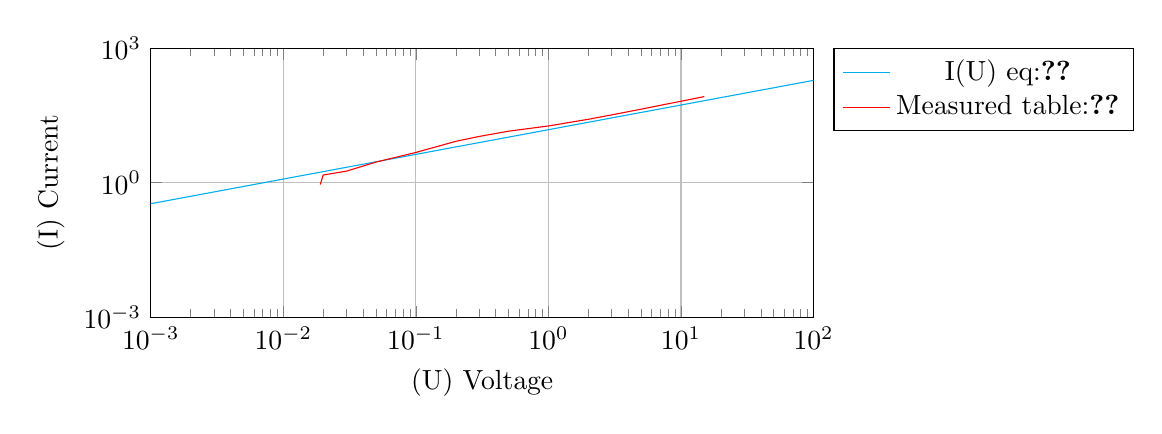
\begin{tikzpicture}
\begin{axis}
[
    xlabel={(U) Voltage},
    ylabel={(I) Current},
    grid,
    width=10cm,
    height=5cm,
    xmin=1e-3, xmax=1e2,
    ymin=1e-3, ymax=1e3,
    xmode=log, ymode=log,
    log basis x=10,
    legend pos=outer north east
    % x filter/.code=\pgfmathparse{#1 + 6.90775527898214},
    % y filter/.code=\pgfmathparse{#1 + 6.90775527898214},
    % log ticks with fixed point,
]
\addplot[cyan, no marks, domain=1e-6:1e2, samples=50] {15.22*x^0.55};
\addlegendentry{I(U) eq:\(\ref{eq:i-u-power-function}\)}
\addplot[red, no marks, domain=1e-6:1e2, samples=50] table {
0.019 0.911
0.020 1.487
0.030 1.816
0.050 2.886
0.100 4.735
0.200 8.381
0.300 10.766
0.500 14.090
1.000 18.450
2.000 25.980
3.000 32.560
5.000 43.660
8.000 57.570
9.000 61.700
10.000 65.680
11.000 69.400
12.000 73.060
13.000 76.580
14.000 79.970
15.000 83.280
};
\addlegendentry{Measured table:\(\ref{bulb-measurements}\)}
\end{axis}
\end{tikzpicture}
\caption{\label{i-u-kennlinie}I-U-Kennlinie.}
\end{figure}

\newpage
\section[Ohmmeter]{Widerstandsmessung mittels Ohmmeter}
\subsection{Versuchsbeschreibung}
Nun wird der Widerstand der Glühbirne zum Abgleich mit den gemessenen Widerständen aus der Vermessung mittels spannungs- und stromrichtiger Messung \ref{experimental-measurements} mittels eines Ohmmeters bestimmt. Dies geschieht mittels eines analogen Multimeters und eines digitalen Multimeters \textit{METRAHit TECH}.

\subsection{Messdaten}

\begin{table}[!h]
    \centering
    \begin{tabular}{@{}rr@{}}
    \toprule
    Device & (R) Resistance\\
    \midrule
        METRAHit TECH & 20.8\si{\ohm}\\
        Analog Unigor & 21\si{\ohm}\\
    \bottomrule
    \end{tabular}
    \caption{\label{bulb-measurements}Glühlampen-Vermessung.}
\end{table}

\section{Auswertung}

Bei Betrachtung der jeweiligen Gerade der berechneten Erwartungswerte und die der Messwerte wird eindeutig, dass diese sehr nah beieinander liegen. Daher bestätigt dies die Formel \ref{eq:i-u-power-function} zur Näherung der Glühbirne. Zur Ermittlung der Formel mit unseren Messwerten bzw. mit der Ausgleichsgeraden, werden die Werte \(a\) \& \(b\) wie folgt bestimmt:

\begin{align}
    \begin{split}
        I_M &= a \cdot U_M^b\\
    \end{split}
\end{align}
wobei \(U_M = 0.976\si{\volt} \approx 1\si{\volt}\) (siehe Tabelle \ref{bulb-measurements}) und \(b \in \mathbb{R}\).
\begin{align}
    \begin{split}
        \therefore \quad I_M &= a \cdot 1^b\\
        &= a \cdot 1\\
        a &= I_M\\
    \end{split}
\end{align}
wobei \(I_M = 18.450\si{\milli\ampere}\).
\begin{align}
    \begin{split}
        \therefore \quad a &= 18.45\\
    \end{split}
\end{align}

\begin{align}
    \begin{split}
        I_M &= a \cdot U_M^b\\
        b &= \frac{\log_{10} I_M - log_{10} a}{log_{10} U_M}
    \end{split}
\end{align}
wobei \(U_M = 9.9\si{\volt} \approx 10\si{\volt}\) und \(I_M = 65.68\si{\milli\ampere}\) (siehe Tabelle \ref{bulb-measurements}).
\begin{align}
    \begin{split}
        \therefore \quad b &= \frac{\log_{10} \left(65.68\right) - log_{10} \left(18.45\right)}{log_{10} \left(10\right)}\\
        &\approx 0.551
    \end{split}
\end{align}
Der Wert \(b\) ist nahezu identisch zum vorgegebenen Näherungswert. Der Wert \(a\) weicht allerdings  um 21.38\% ab.

\begin{table}[!h]
    \centering
    \begin{tabular}{@{}rrrrrrrrr@{}}
    \toprule
    ~ & \multicolumn{2}{c}{Measurements} & \multicolumn{1}{c}{Derived}\\
    Target & (\(I\)) Current & (\(U\)) Voltage & (\(R_A\)) Resistance\\
    \midrule
    10\si{\milli\volt} & 0.911\si{\milli\ampere} & 0.019\si{\volt} & 20.85620\si{\ohm}\\
    100\si{\milli\volt} & 4.735\si{\milli\ampere} & 0.102\si{\volt} & 21.54171\si{\ohm}\\
    300\si{\milli\volt} & 10.766\si{\milli\ampere} & 0.290\si{\volt} & 26.93665\si{\ohm}\\
    2\si{\volt} & 25.980\si{\milli\ampere} & 1.996\si{\volt} & 76.82832\si{\ohm}\\
    5\si{\volt} & 43.660\si{\milli\ampere} & 4.920\si{\volt} & 112.68896\si{\ohm}\\
    10\si{\volt} & 65.680\si{\milli\ampere} & 9.900\si{\volt} & 150.73081\si{\ohm}\\
    \bottomrule
    \end{tabular}
    \caption{\label{r-a-calculation}\(R_A\)-Berechnung.}
\end{table}
Vergleicht man die Gleichstromwiderstände, ist zu erkennen, dass bei kleinen Spannungen die Werte noch nah an den Werten der Ohmmeter liegen. Hier stimmen die Ströme, mit denen die Ohmmeter messen, mit den der Messreihe überein. Da die Glühbirne ein nicht linearer Widerstand ist, gehen die Werte bei höheren Spannungen auseinander.

Die differentiellen Widerstände ergeben sich aus dem Kehrwert der Ableitung der Formel.

\begin{table}[!h]
    \centering
    \begin{tabular}{@{}rrrrrrrrr@{}}
    \toprule
    Target & (\(R_d\)) Expected & (\(R_d\)) Measured & rel. Error\\
    \midrule
    10\si{\milli\volt} & 0.015\si{\ohm} & 0.012\si{\ohm} & 0.174\\
    100\si{\milli\volt} & 0.042\si{\ohm} & 0.035\si{\ohm} & 0.176\\
    300\si{\milli\volt} & 0.070\si{\ohm} & 0.057\si{\ohm} & 0.177\\
    2\si{\volt} & 0.163\si{\ohm} & 0.134\si{\ohm} & 0.178\\
    5\si{\volt} & 0.247\si{\ohm} & 0.203\si{\ohm} & 0.179\\
    10\si{\volt} & 0.337\si{\ohm} & 0.277\si{\ohm} & 0.180\\
    \bottomrule
    \end{tabular}
    \caption{\label{differential-resistances}Differentielle Widerstände.}
\end{table}

\chapter{Ersatzquellen}

\section{Messung Original-Schaltung}
\subsection{Versuchsbeschreibung}
Für ein Widerstandsnetzwerk mit zwei Spannungsquellen soll rechnerisch und experimentell eine
Ersatzquelle bestimmt werden, die sich bezüglich der Klemmen \textbf{a} und \textbf{b} genau wie das
ursprüngliche Netzwerk verhält.

Das Netzwerk \ref{fig:original-circuit} soll verschaltet werden und \(R_7\) soll zunächst \textbf{nicht} angeschlossen werden.
Als Spannungsquelle wird das Labornetzgerät \textit{Hameg Triple Power Supply HM7042-5} verwendet.

\[
U_1 = U_2 = 4.5V
\]
\[
R_1 = 1k\Omega, R_2 = 100\Omega, R_3 = 220\Omega, R_4 = 680\Omega, R_7 = 470\Omega.
\]

\subsection{Schaltplan}

\begin{figure}[!h]\centering
\begin{circuitikz}[american, scale = 0.7]
\draw
(0,0) to[european voltage source, l=$U_1$] (0,4) -- (0,8)
      to[resistor, l=$R_1$, -*] (4,8)
      to[resistor, l=$R_2$] (4,4)
      to[european voltage source, l=$U_2$] (4,0) -- (0,0)

(4,8) to[resistor, l=$R_3$] (8,8) -- (8,6)
      to[resistor, l=$R_4$] (8,0) to[short, -*] (4,0)

(8,6) to[short, *-o] (9.5,6)
node[label={[font=\footnotesize]above:a}] {}

(10,5.5) to [open,v=$U_{ab}$] (10,0.5)

(10.5,6) to[short, i=$I_7$, o-.] (12,6)
      to[resistor, l=$R_7$] (12,0)
      to[short, .-o] (10.5,0)

(9.5,0)
node[label={[font=\footnotesize]above:b}] {}

(9.5,0) to[short, o-*] (8,0)

(12,4.5) -- (14,4.5)
      to[voltmeter] (14,1.5) -- (12,1.5)
(14.3,3) node[label={[font=\footnotesize]east:$U_{R_7}$}] {}

(0,0) to[short, *-] (0,-0.5) node[ground]{};
;
\end{circuitikz}
\caption{Original-Schaltung} \label{fig:original-circuit}
\end{figure}

\subsection{Vorbereitung}
Es werden folgende vorbereitende Berechnungen durchgeführt:

\paragraph{Berechnung der Innenwiderstandes $R_i$}\mbox{}\\
Umformung des Original Schaltkreises \ref{fig:original-circuit}.

\begin{figure}[!h]\centering
\begin{circuitikz}[american, scale = 0.7]
\draw

(0,3) node[label={[font=\footnotesize]above:a}] {}
(0,3) to[short, o-*] (2,3)

(2,3) -- (2,5)
    to[resistor, l=$R_4$] (12,5)
    to[short, -*] (12,3)

(2,3) -- (2,1)
    to[resistor, -*, l=$R_3$] (6,1)

(6,1) -- (6,2)
    to[resistor, l=$R_1$] (10,2)
    to[short, -*] (10,1)

(6,1) -- (6,0)
    to[resistor, l=$R_2$] (10,0) -- (10,1)

(10,1) -- (12,1) -- (12,3)
    to[short, -o] (14,3)

(14,3) node[label={[font=\footnotesize]above:b}] {}
;
\end{circuitikz}
\caption{Innenwiderstands-Schaltkreis} \label{fig:r-i-circuit}
\end{figure}

\begin{align}
R_{1||2} &= \left[\frac{1}{R_1}+\frac{1}{R_2}\right]^{-1}
= \left[\frac{1}{1000\Omega}+\frac{1}{100\Omega}\right]^{-1}
= \frac{1000}{11}\Omega
\approx 90.91\Omega\\
R_{\left(1||2\right)+R_3} &= R_{1||2} + R_3 = \frac{1000}{11}\Omega + 220\Omega = 310.91\Omega\\
R_i = R_{\left[\left(1||2\right)+R_3\right]||R_4} &= \left[\frac{1}{R_{\left(1||2\right)+R_3}}+\frac{1}{R_4}\right]^{-1}
= 310.91\Omega + 680\Omega = 213.36\Omega
\end{align}

\paragraph{Berechnung der Leeflaufspannung $U_L$}\mbox{}\\
Leerlaufspannung $U_L$ (ohne Belastung mit $R_7$) wird mittels der Superpositionsprinzip berechnet.

\[
U_L = U_{ab} =  U_{4,2} + U_{4,1}
\]

\subparagraph{Einfluss von $U_1$:}
Alle Teilspannungen \& Teilströme sind in Bezug auf $U_1$ als Gesamtspannung und $I_1$ als Gesamtstrom.

\begin{align}
R_{g1} &= R_4 + \left[ \frac{1}{R_2} + \frac{1}{R_3 + R_4} \right]^{-1}
= 1,090\Omega\\
I_{1} &= \frac{U_1}{R_{g1}} = \num{4.128e-3}\si{\ampere}\\
\intertext{Nun wird der Spannungsabfall über der Masche $R_3$ + $R_4$ berechnet.}
U_{R_3+R_4} &= U_1 - \left( I_1 \cdot R_1 \right) \approx 0.372\si{\volt}
\intertext{Nun wird der Spannungsabfall über $R_4$ mittels des Spannungsteilers berechnet.}
U_{4,1} &= U_{R_3+R_4} \cdot \frac{R_4}{R_3 + R_4} \approx 0.281\si{\volt}
\end{align}


\subparagraph{Einfluss von $U_2$:}
Alle Teilspannungen \& Teilströme sind in Bezug auf $U_2$ als Gesamtspannung und $I_2$ als Gesamtstrom.

\begin{align}
R_{g2} &= R_2 + \left[ \frac{1}{R_1} + \frac{1}{R_3 + R_4} \right]^{-1}
= 573.68\Omega\\
I_{2} &= \frac{U_2}{R_{g2}} = \num{7.844e-3}\si{\ampere}\\
\intertext{Nun wird der Spannungsabfall über der Masche $R_3$ + $R_4$ berechnet.}
U_{R_3+R_4} &= U_2 - \left( I_2 \cdot R_2 \right) \approx 3.716\si{\volt}
\intertext{Nun wird der Spannungsabfall über $R_4$ mittels des Spannungsteilers berechnet.}
U_{4,2} &= U_{R_3+R_4} \cdot \frac{R_4}{R_3 + R_4} \approx 2.808\si{\volt}
\end{align}

\subparagraph{Kombination der einzelnen Einflüsse von $U_1$ und $U_2$:}
\begin{align}
\begin{split}
U_{ab} &= U_{4,1} + U_{4,2}\\
&= 0.281\si{\volt} + 2.808\si{\volt}\\
&= 3.089\si{\volt}
\end{split}
\end{align}

\paragraph{Berechnung der Kurzschlussstromes $I_K$}\mbox{}\\

\begin{align}
\begin{split}
I_K &= I_{ab} = \frac{U_{ab}}{R_i} = \frac{U_{L}}{R_i}\\
&= \frac{3.089\si{\volt}}{213.36\si{\ohm}}\\
&\approx 0.014\si{\ampere}
\end{split}
\end{align}

\paragraph{Berechnung der Klemmenspannung $U_{R_7}$}\mbox{}\\
Klemmenspannung $U_{R_7}$ bei Belastung mit $R_7$

\begin{align}
\begin{split}
U_{R_7} &= U_{ab} \cdot \frac{R_7}{R_i + R_7}\\
&= 3.089\si{\volt} \cdot \frac{470\si{\ohm}}{213.36\si{\ohm} + 470\si{\ohm}}\\
&\approx 2.125\si{\volt}
\end{split}
\end{align}

\paragraph{Berechnung des Laststromes $I_7$}\mbox{}\\
Laststrom $I_{R_7}$ bei Belastung mit $R_7$

\begin{align}
\begin{split}
I_{R_7} &= \frac{U_{ab}}{R_i + R_7}\\
&= \frac{3.089\si{\volt}}{213.36\si{\ohm} + 470\si{\ohm}}\\
&\approx \num{4.52e-3}\si{\ampere}
\end{split}
\end{align}

\subsection{Durchführung}
Der Original-Schaltkreis \ref{fig:original-circuit} wurde auf dem Steckboard aufgebaut. Das Labornetzgerät \textit{Hameg Triple Power Supply HM7042-5} wurde auf die Spannungen \(U_1 = U_2 = 4.5\si{\volt}\) eingestellt. Die Leerlaufspannung \(U_L\) wurde mit dem Digitalmultimeter \textit{METRAHit 15S} an den Klemmen \textbf{a} und \textbf{b} ohne den Lastwiderstand \(R_7\) gemessen. Der Kurschlussstrom \(I_K\) wurde mit einem digitales Amperemeter \textit{METRAHit TECH 18s} an den Klemmen \textbf{a} und \textbf{b} gemessen.

\subsection{Messdaten}

\begin{table}[!h]
    \centering
    \begin{tabular}{@{}rrr@{}}
    \toprule
    ~ & Calculated Value & Measured Value\\
    \midrule
        \(U_{ab}\) & 3.089\si{\volt} & 3.11\si{\volt} \\
        \(I_K\) & 14\si{\milli\ampere} & 14.5\si{\milli\ampere} \\
        \(U_{R_7}\) & 2.125\si{\volt} & 2.136\si{\volt} \\
        \(I_{R_7}\) & 4.52\si{\milli\ampere} & 4.556\si{\milli\ampere} \\
    \bottomrule
    \end{tabular}
    \caption{\label{original-circuit-measurements}Original-Schaltungs-Vermessung.}
\end{table}

\section{Messung Ersatz-Schaltung}
\subsection{Versuchsbeschreibung}
Das Widerstandsnetzwerk \ref{fig:original-circuit} links von den Klemmen \textbf{a} und \textbf{b} soll durch eine Ersatzschaltung \ref{fig:ersatz-circuit} ersetzt werden. Der Innenwiderstand links von den Klemmen \textbf{a} und \textbf{b} liegenden Widerstandsnetzwerk \ref{fig:original-circuit} wird aus der Vorbereitungsrechnung bezogen.
\[
R_i = R_{\left[\left(1||2\right)+R_3\right]||R_4} = \left[\frac{1}{R_{\left(1||2\right)+R_3}}+\frac{1}{R_4}\right]^{-1}
= 310.91\Omega + 680\Omega = 213.36\Omega
\]
Die Schaltung soll aufgebaut werden mit Hilfe eines einstellbaren Netzteiles \textit{Hameg Triple Power Supply HM7042-5} und einer Widerstandsdekade. Es sind die Werte für \(U_L\) und \(R_i\) aus der Vorbereitungsrechnung einzustellen. Leerlaufspannung \(U_L\) und Kurzschlussstrom \(I_K\) sind an den Klemmen \textbf{a} und \textbf{b} zu messen.

Im Folgenden wird der Widerstand \(R_7\) angeschlossen und der durch ihn fließende Strom \(I_7\) und die anliegende Spannung \(U_{R_7}\) wird gemessen.

\newpage
\subsection{Skizze}

\begin{figure}[!h]\centering
\begin{circuitikz}[american, scale = 0.7]
\draw
(0,0) to[european voltage source, l=$U_0$] (0,4) -- (0,8)
      to[resistor, l=$R_i$, -] (4,8)

(4,8) to[short] (8,8) -- (8,6)

(8,6) to[short, -o] (9.5,6)
node[label={[font=\footnotesize]above:a}] {}

(10,5.5) to [open, v=$U_{ab}$] (10,0.5)

(10.5,6) to[short, i=$I_7$, o-.] (12,6)
      to[resistor, l=$R_7$] (12,0)
      to[short, .-o] (10.5,0)

(9.5,0) node[label={[font=\footnotesize]above:b}] {}

(9.5,0) to[short, o-] (8,0) -- (0,0)

(12,4.5) -- (14,4.5)
      to[voltmeter] (14,1.5) -- (12,1.5)

(14.3,3) node[label={[font=\footnotesize]east:$U_{R_7}$}] {}

(0,0) to[short, *-] (0,-0.5) node[ground]{};
;
\end{circuitikz}
\caption{Ersatz-Schaltung} \label{fig:ersatz-circuit}
\end{figure}

\subsection{Messdaten}

\begin{table}[!h]
    \centering
    \begin{tabular}{@{}rrr@{}}
    \toprule
    ~ & Calculated Value & Measured Value\\
    \midrule
        \(U_{ab}\) & 3.089\si{\volt} & 3.09\si{\volt} \\
        \(I_K\) & 14\si{\milli\ampere} & 14.23\si{\milli\ampere} \\
        \(U_{R_7}\) & 2.125\si{\volt} & 2.118\si{\volt} \\
        \(I_{R_7}\) & 4.52\si{\milli\ampere} & 4.522\si{\milli\ampere} \\
    \bottomrule
    \end{tabular}
    \caption{\label{ersatz-circuit-measurements}Ersatz-Schaltungs-Vermessung.}
\end{table}

\section{Auswertung}

Die Messungen in der Originalschaltung haben ergeben, dass die vorher angefertigten Berechnung korrekt waren.
Durch den Aufbau der Ersatzschaltung \ref{fig:ersatz-circuit} konnte gut dargestellt werden, dass die Schaltung \ref{fig:original-circuit} (Originalschaltung) durch den errechneten Ersatzwiderstand \(R_i = 213.36\si{\ohm}\) nachgestellt werden kann.

Auch die Messungen am angeschlossenen Widerstand \(R_7\) in der Ersatzschaltung waren identisch zur Messung am Widerstand \(R_7\) in der Originalschaltung.
Die Abweichung sind \(<\num{1e-2}\) weshalb diese zu vernachlässigen sind.

Die geringen Abweichungen (\(<\num{1e-1}\)) der Berechnung erklären wir uns durch nicht berücksichtige Leiterwiderstände in der Rechnung.

\chapter{Auswertung}

Die Zielsetzung konnte anhand der Experimente gut erfüllt werden.
Es sind Erkenntnisse über die sinnvolle Anwendung der Messmethoden gewonnen worden und das Verständnis von Ersatzquellen konnte durch Abgleichen der Messung mit den Berechnungen gefestigt werden.

Die Auswertung aus den Versuchen führen zu folgenden Erkenntnissen:
\begin{itemize}
  \item Eine Messung von kleinen Widerständen mittels Multimeter ist sehr ungenau.
  \item Leiterwiderstände haben einen großen Einfluss bei kleinen Widerständen.
  \item Analoge Multimeter sind deutlich fehleranfälliger als Digitale Multimeter.
  \item Stromrichtiges Messen ist besser geeignet für das Messen von großen Widerständen.
  \item Spannungsrichtiges Messen ist besser geeignet für das Messen von kleinen Widerständen.
  \item Zwei-Punkt-Methode sorgt bei kleinen Widerständen für sehr große Abweichung, die Vier-Punkt-Methode ist besser geeignet.
  \item Zwei- und Vier-Punkt-Methode verhalten sich beim Messen des 1kOHM Widerstandes nahezu identisch.
  \item Nichtlineare Widerstände stimmen nur bei sehr kleinen Strömen mit den Messungen eines Ohmmeters überein.
  \item Temperatur hat hier einen Einfluss auf den nichtlinearen Widerstand.
  \item Eine Schaltung kann durch die Berechnung des Innenwiderstands in eine Ersatzschaltung umgebaut werden.
  \item Die Messwerte in der Ersatzschaltung sind identisch zur Originalschaltung.
\end{itemize}
Für die nächsten Praktika empfiehlt es sich, parallel zur Versuchsdurchführung, ein Gruppenmitglied zur direkten Diagramm Erstellung zu beauftragen, um mögliche Messfehler oder anderweitige Abweichungen schnell erkennen zu können.
Zudem können sofort erste Erkenntnisse gewonnen werden, was die Erstellung des Berichtes vereinfacht.

\bibliographystyle{abbrv}
% \bibliography{references}  % need to put bibtex references in references.bib
\end{document}